\documentclass[tikz]{standalone}%

\usepackage[utf8]{inputenx}%  http://ctan.org/pkg/inputenx
% Euler for math | Palatino for rm | Helvetica for ss | Courier for tt
\renewcommand{\rmdefault}{ppl}% rm
\linespread{1.05}% Palatino needs more leading
\usepackage[scaled]{helvet}% ss //  http://ctan.org/pkg/helvet
\usepackage{courier}% tt // http://ctan.org/pkg/courier
\usepackage{eulervm}  %  http://ctan.org/pkg/eulervm
% a better implementation of the euler package (not in gwTeX)
\normalfont%
\usepackage[T1]{fontenc}%  http://ctan.org/pkg/fontenc
\usepackage{textcomp}%  http://ctan.org/pkg/textcomp

\usetikzlibrary{calc}
\usetikzlibrary{intersections}
\usetikzlibrary{angles}
\usetikzlibrary{quotes}

\begin{document}
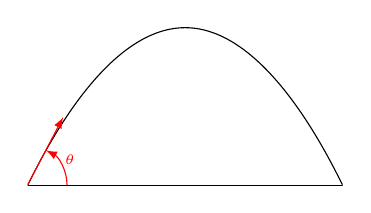
\begin{tikzpicture}
  \clip (0, 0) rectangle (4, 2);

  \coordinate (O) at (0, 0);
  
  \path[name path = para] (-1, -2.5) parabola bend (2, 2) (4, 0);
  
  \draw (O) parabola bend (2, 2) (4, 0);
  \draw (O) -- (4, 0) coordinate (P1);

  \path[name path = circ] (O) circle[radius = .75bp];
  \path[name intersections = {of = para and circ}];

  \coordinate (A) at (intersection-1);
  \coordinate (B) at (intersection-2);

  \draw[-latex, red] (B) -- ($(B)!1cm!(A)$) coordinate (P2);

  \path (P1) -- (O) -- (P2)
  pic["$\theta$", draw, -latex, red, angle radius = .5cm,
  angle eccentricity = 1.25, font = \tiny] {angle = P1--O--P2};
\end{tikzpicture}
\end{document}
%%% Local Variables:
%%% mode: latex
%%% TeX-master: t
%%% End:
